% Exemple d'utilisation de la classe `thesul' pour un master.
% D. Roegel, 3/4/2013
%
% Note : les couvertures de Master ne sont pas finalisées dans thesul.
%        Indiquez-moi ce qu'il faut mettre.
%
\documentclass{thesul}
\usepackage{capt-of}
\usepackage{lipsum}% just to generate text for the example
\usepackage{placeins}



%-------------------------------------------------------------------
%                         Les références
%-------------------------------------------------------------------

\NoChapterNumberInRef
\NoChapterPrefix


\begin{document}

      \OddHead={{\leftmark\rightmark}{\hfil\slshape\rightmark}}
      \EvenHead={{\leftmark}{{\slshape\leftmark}\hfil}}
      \OddFoot={\hfil\thepage}
      \EvenFoot={\thepage\hfil}
      \pagestyle{ThesisHeadingsII}

%-------------------------------------------------------------------
%            Réinitialisation de la numérotation des chapitres
%-------------------------------------------------------------------

% Si la commande suivante est présente,
% elle doit figurer APRÈS \begin{document}
% et avant la première commande \part
\ResetChaptersAtParts 





\MasterUL
\ThesisTitle{Formal Verification of Distributed Algorithms using Distributed-PlusCal}
\ThesisAuthor{Heba Al-kayed}
\ThesisPresentedThe{soutenu le 23 septembre 2016}
\President    = {Le pr\'esident}
\Rapporteurs  = {Le rapporteur 1\\
                 Le rapporteur 2\\
                 Le rapporteur 3}
\Examinateurs = {L'examinateur 1\\
                 L'examinateur 2}

\MakeThesisTitlePage


%-------------------------------------------------------------------
%                          remerciements
%-------------------------------------------------------------------

%\DontFrameThisInToc
\begin{ThesisAcknowledgments}
Les remerciements.
\end{ThesisAcknowledgments}

%-------------------------------------------------------------------
%                            dédicace
%-------------------------------------------------------------------

\begin{ThesisDedication}
Je dédie cette thèse\\
à ma machine.\\
Oui, à Pandore,\\
qui fut la première de toutes.
\end{ThesisDedication}


%-------------------------------------------------------------------
%                  écriture de `Chapitre' et `Partie' 
%                      dans la table des matières
%-------------------------------------------------------------------

\WritePartLabelInToc
\WriteChapterLabelInToc

%-------------------------------------------------------------------
%                        table des matières
%-------------------------------------------------------------------

\tableofcontents

% Pour ne pas avoir le mot « Chapitre » au début de chaque chapitre.
\NoChapterHead


% La commande \mainmatter permet de passer
% à la numérotation arabe (ce que fait \pagenumbering{arabic}) 
% et de faire commencer la nouvelle page 1 sur une page impaire.
% On évitera donc d'utiliser directement \pagenumbering{arabic}.
\mainmatter


\chapter{Introduction}
%%============================
This is a very nice thesis about TLA~\cite{tlabook}.

\paragraph*{Motivations}
why this extension

\paragraph*{Outline}


\chapter{Background info}
%%============================

a brief overview of ModelChecking, TLA and Pluscal possibly with an example to show why it's used or its advantages.
maybe mention real life applications like amazon's AWS.


\section{TLA+}
%%============================

\cite{tlabook}.

\section{PlusCal algorithm language}
%%============================
 

\chapter{Related work}
%%============================
position of our work compared with other work

\section{PGO}

\subsection{Modular PlusCal}

\chapter{Distributed PlusCal}

Writing a distributed algorithm is not an easy task which is why most programming languages provide supporting primitives that make this process a bit easier for the programmer, in Distributed PlusCal we as well introduced some of these supporting primitives such as threads and communication channels.

Both PlusCal and Distributed PlusCal translators expect a file with a '.tla' extension, an algorithm that starts with '--algorithm', and the decleration of variables and processes, so there are not many differences in the structure of the file itself, we have added an option to the options in PlusCal with the name 'distpcal', the presence of this option is considered the enabler of the Distributed PlusCal translator and once it's found in the options statement then our translator will be the one doing the parsing regardless of the actual content of the PlusCal statements present in the file.

\section{Threads}

A PlusCal process consists of two parts, a variable deceleration part and part that holds the statements to be executed when the process is running.
Distributed PlusCal gives each process the opportunity to define more than one part to hold statements to be executed, that is if we consider the first   block to be the main thread of a process, then we can think about the added blocks as threads that run in parallel with the main block.

This enables the process to be executing multiple tasks in parallel, for example a thread can be used to send/receive data to/from other processes asynchronously while the main thread is executing it's statement uninterrupted by such commands.

\hfill\\
The body of a thread maintains all the same properties and syntax as the body of a normal PlusCal block, all the threads share the same variables declared for the process making synchronization between these threads simple and straightforward.


//to be rephrased \hfill\\
Figure \ref{fig:process} shows the general structure of a Distributed PlusCal process written in C-Syntax, the differences between this structure and the structure of a process in PlusCal are the ability to define multiple threads and the fact that a 'process' can also hold the name 'node'.


\begin{figure}[h!]
\centering
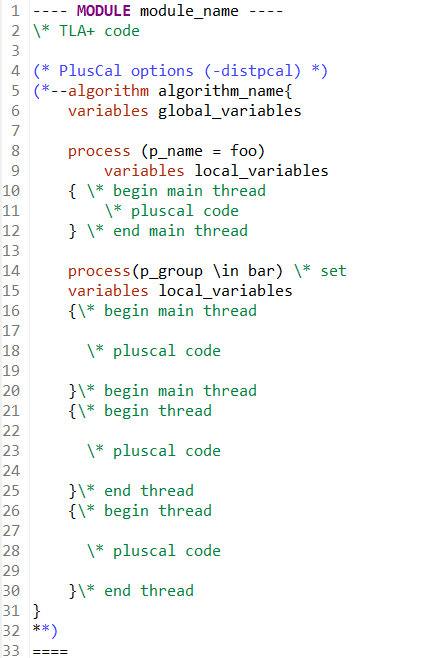
\includegraphics[scale=0.8]{ProcessStruct.png}
\caption{Process Structure}
\label{fig:process}
\end{figure}
\FloatBarrier

\hfill\\
it's important to note that the threads are optional, meaning we can still parse a process with only it's main thread using our translator, also threads do not allow variable declarations they only use variables declared for the entire process.

\subsection{TLA+ Translation}

Defining threads for processes had some effects on the translation to TLA+, because when you declare threads you are actually partitioning the process into multiple sub-parts, so later on whenever we are refering to a process we need to know not only which process it is but also which sub-thread.

Figure \ref{fig:processtla} shows a part of the translation of the Two Phase Commit example.//to be changed to a simpler example 


\begin{figure}[h!]
\centering
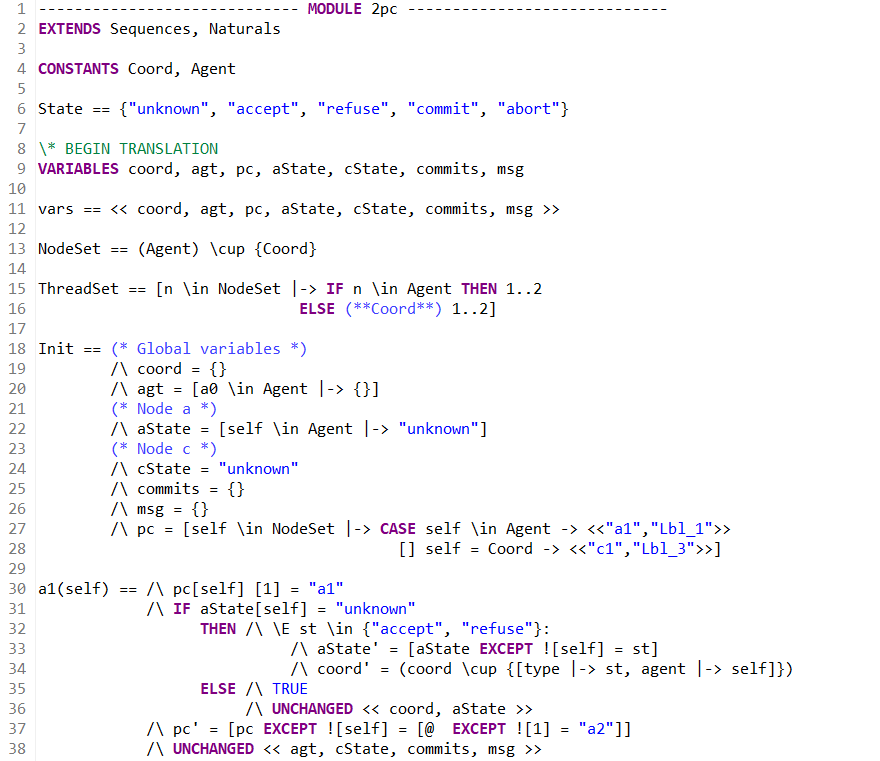
\includegraphics[scale=0.7]{ProcessTLA.png}
\caption{Process Translation}
\label{fig:processtla}
\end{figure}
\FloatBarrier

One of the first things noticeable is the set \textit{NodeSet} at line 18 which is a set of all process identifiers, similarly \textit{ThreadSet} at line 15 is the set of all the thread identifiers per process.

\hfill\\
The \textit{pc} variable in TLA+ that is used to indicate the current point of execution and the next statement to be executed with respect to a process had to now indicate also which sub-part of the process is involved, so we extended it to include information per process per thread.
\hfill\\ At line 27 we initialize the \textit{pc} variable to be a function whose domain is the set of process identifiers and the range consists of a sequence of labels that are considered the entry points per thread.
\hfill\\ Lines 30 and 37 give a clear idea of how the \textit{pc} is expected to be used within the translation.


\section{Channels}
\subsection{Unordered channels}
example with it's translation
\subsection{FIFO channels}
example with it's translation
\subsection{Supported channel functions}
expected syntax and limitations
\subsection{Walk through of the two phase commit example and its translation}
our examples with their translations

\chapter{Code Documentation}

\section{general structure of the toolbox and it's components}
try to describe the general flow

\section{parsing and expansion process}

\section{some software-based diagram}

or maybe an AST description graph

\chapter{Conclusion and future work}
\bibliographystyle{alpha}
\bibliography{report}

\end{document}
